\documentclass[twoside]{article}
\usepackage{package}
\usepackage[T1]{fontenc}
% Silenciar la advertencia de versalita + negrita inexistente
\WarningFilter{latex}{Some font shapes were not available}
\WarningFilter{latex}{Font shape `T1/lmr/bx/sc'}

% Silenciar la advertencia de caracteres perdidos en el nullfont (para 01_introduccion.tex)
\WarningFilter{latex}{Missing character: There is no}
%Nuevos comandos
\renewcommand{\thefootnote}{\arabic{footnote}}
\raggedbottom



\begin{document}
\begin{center}
    \thispagestyle{empty}
    \large{\textsc{Modelos simples en Matlab-Simulink e Interacción Matlab-Simulink}}\\[0.5cm] 
    \large{Fabrizio Benavidez\footnote[1]{\texttt{fabrizio.benavidez@mi.unc.edu.ar}}}\\[0.5cm]

    \large{\footnotemark[1]\textit{Facultad de Ciencias Exactas, Físicas y Naturales, Ingeniería Aeronáutica}}
    \\[0.5cm]

    \begin{minipage}{0.7\textwidth}
    \hrule
    \vspace{0.2cm}
        \normalsize{\textsc{Resumen}. En el presente informe se aborda el modelado y la simulación de sistemas dinámicos continuos descritos por ecuaciones diferenciales ordinarias y funciones de transferencia mediante Matlab\textregistered\ y Simulink\textregistered. Se analiza la respuesta temporal ante diferentes entradas y el comportamiento de sistemas de primer y segundo orden. Asimismo, se explora la interacción entre el entorno de diagramas de bloques y el espacio de trabajo de Matlab (Workspace) para la extracción de datos y personalización de gráficas.}\\[0.2cm]
        
        \normalsize{\textit{Palabras claves}: Simulink, Matlab, Ecuaciones diferenciales, Funciones de transferencia. \ }
    \vspace{0.2cm}
    \hrule
    \end{minipage}
    
    \vfil

    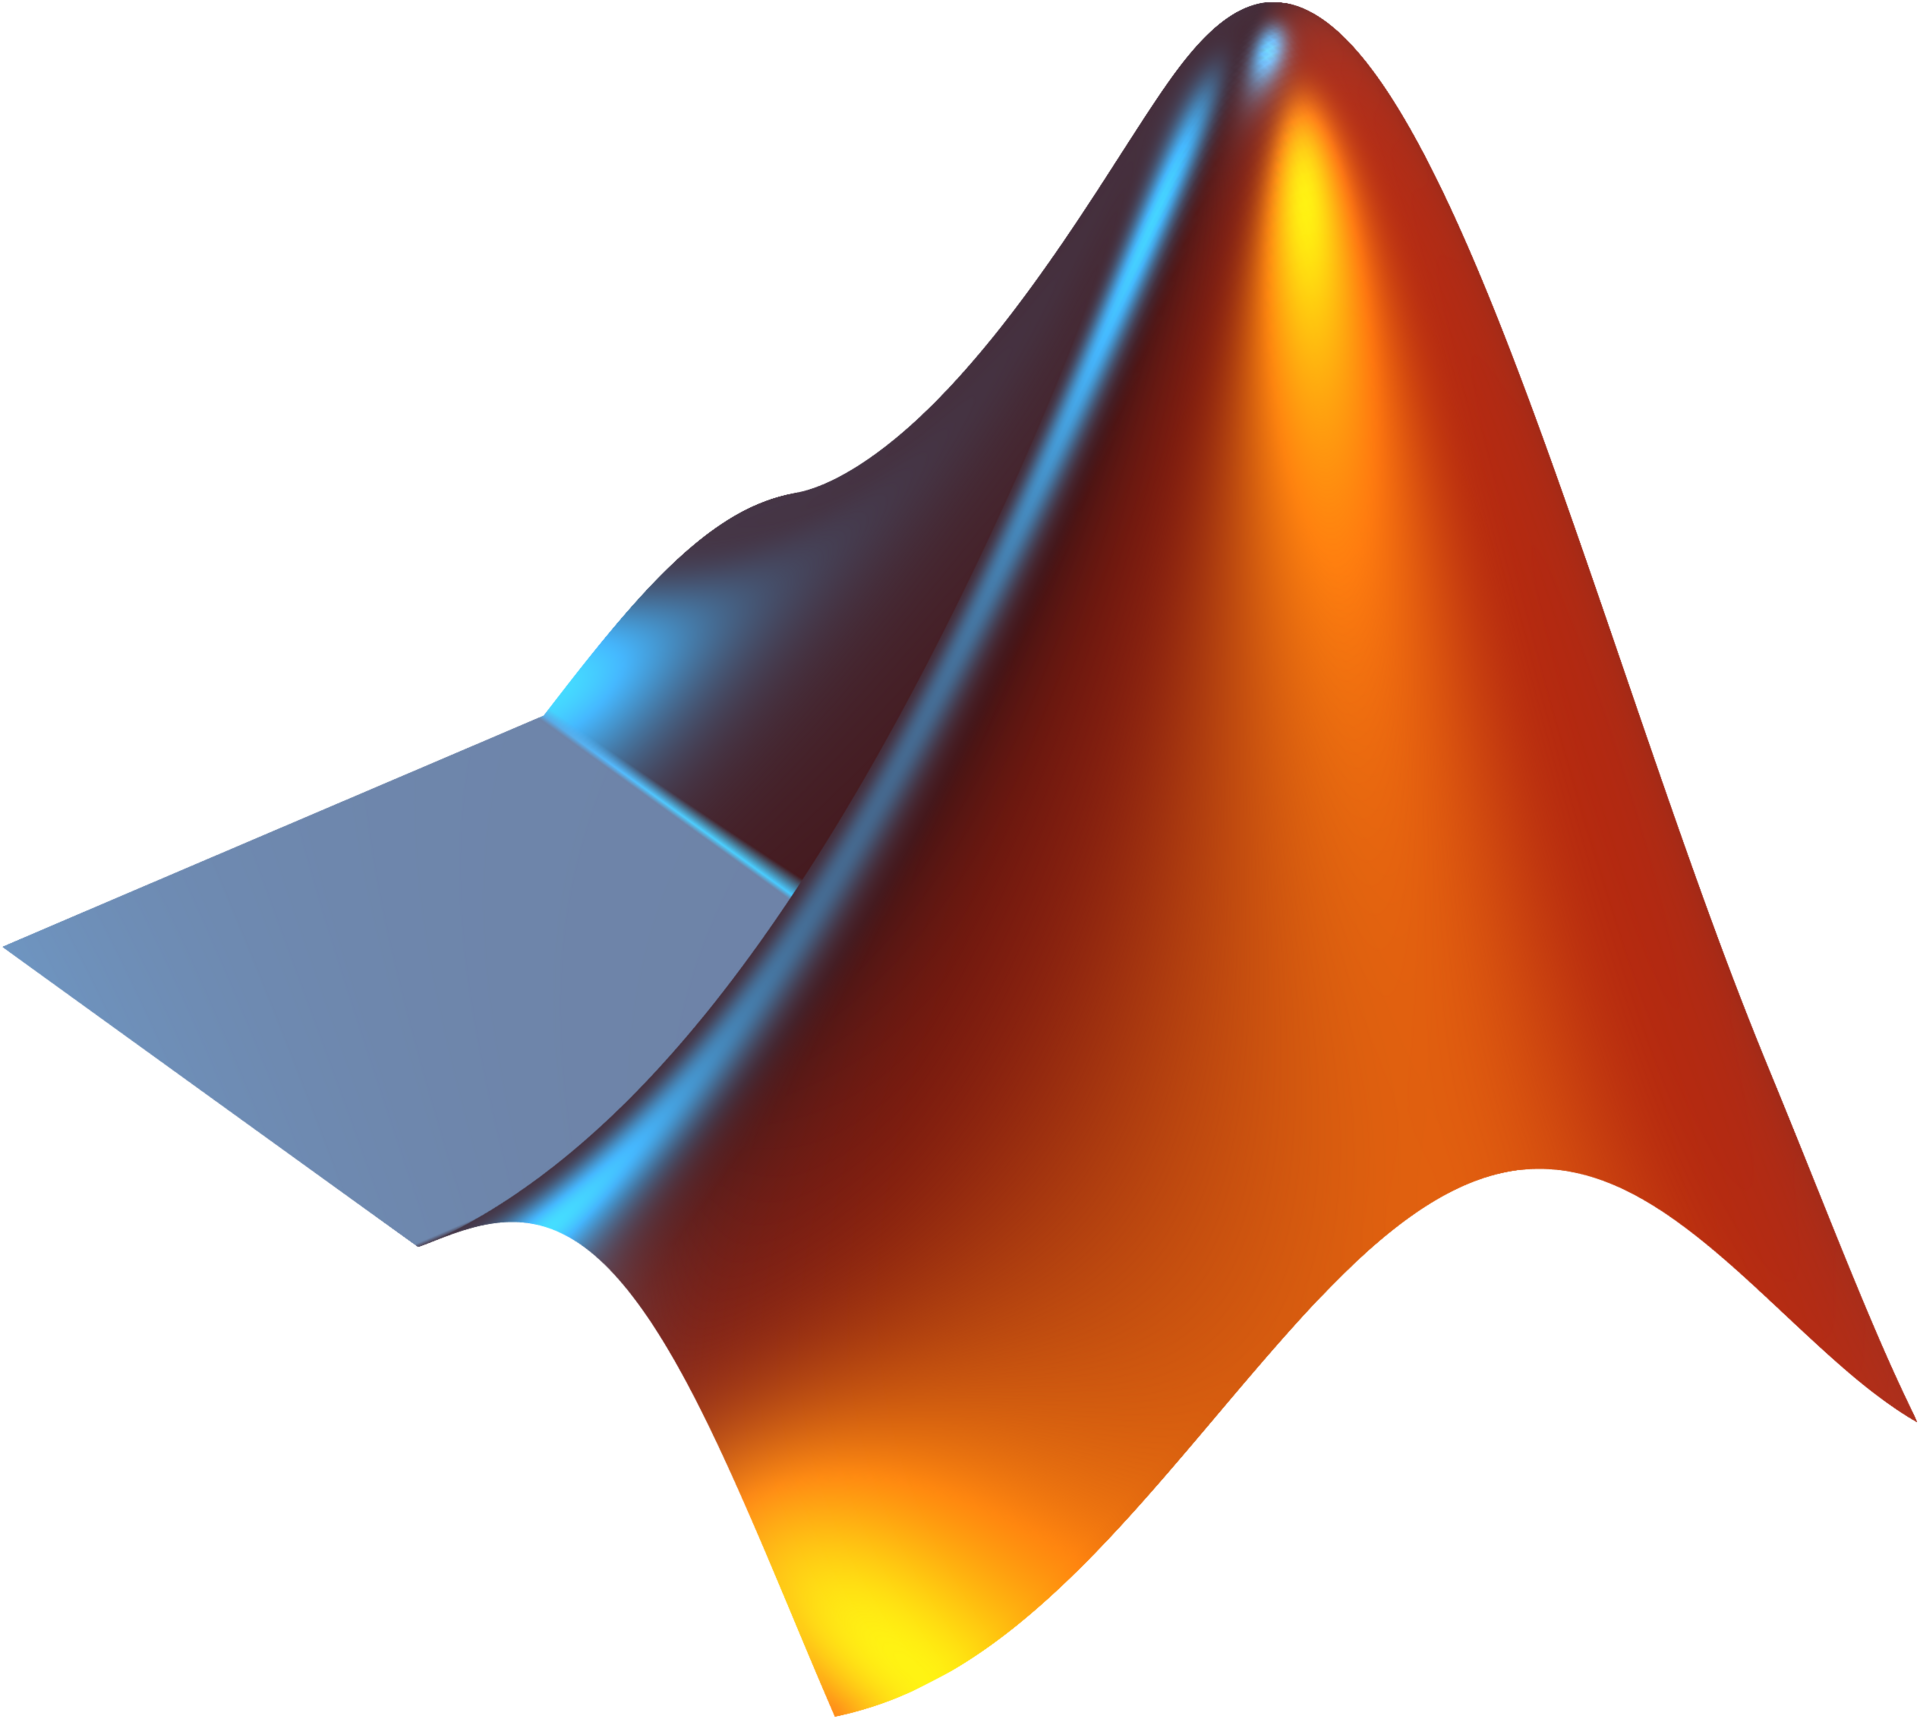
\includegraphics[width = 0.4\textwidth]{imagenes/Matlab_Logo.png}\\[0.5cm]

    \vfil

    \today\\[0.2cm]
    \large{Semana 1}
\end{center}




\newpage



\section{Guía 01}


El sistema 

\begin{equation*}
    \dot{x} = 3r(t)
\end{equation*}

\noindent donde $r(t) = H(t)$, siendo $H(t)$ la función de Heaviside o función escalón. El diagrama de bloques de la siguiente ecuación diferencial es  

\begin{figure}[ht!]
    \centering
    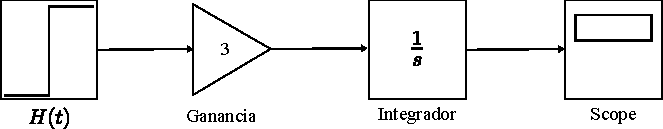
\includegraphics[width = 0.7\textwidth]{imagenes/diagrame_en_bloque.pdf}
    \caption{Diagrama en bloques de la ecuación diferencial}
    \label{fig:1}
\end{figure}


\noindent Una vez creada este diagrama en bloques en \textit{Simulink}, podemos darle a \textbf{Run} y hacer doble click en \textbf{Scope}. Para manipular el bloque \textbf{Step}, se puede hacer doble click en el bloque y poner en \textbf{Step time} $= 2$. Para la condición inicial se hace exactamente igual pero en la parte de \textbf{Initial value}. Por lo tanto, para una respuesta de 20 segundos con una entrada escalón a $1$ s y $2$ s, se obtiene la siguiente figura.

\begin{figure}[ht!]
    \label{fig:2}
    \begin{center}
        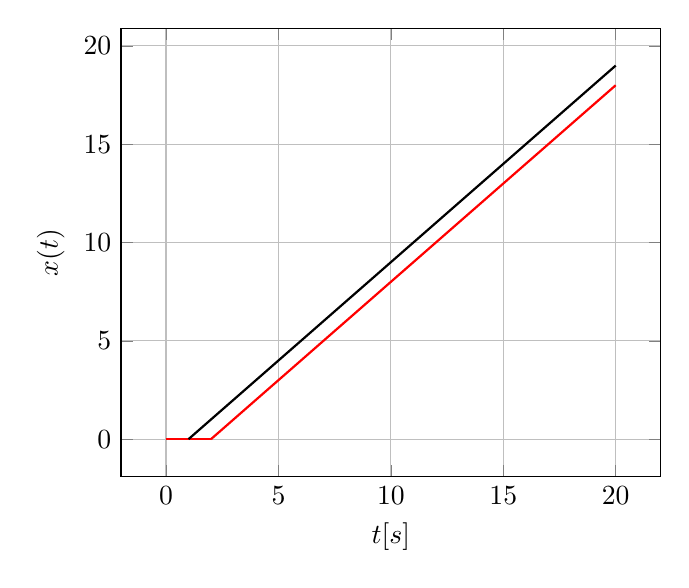
\begin{tikzpicture}
            \begin{axis}[grid,
                xlabel = {$t [s]$},
                ylabel = {$x(t)$}]
                \addplot[domain = 0:1, thick]{0};
                \addplot[domain = 0:2, thick, red]{0};
                \addplot[domain = 1:20, thick]{x-1};
                \addplot[domain = 2:20, thick, red]{x-2};
            \end{axis}
        \end{tikzpicture}
    \end{center}
    \caption{Salida $x(t)$ por una función escalón}
\end{figure}



Dado el sistema:

\begin{equation*}
    \dot{x}(t) = t + 7 - 4x(t)
\end{equation*}


\noindent Su diagrama en bloques se puede construir mediante un \textit{Constant}, \textit{Clock}, \textit{Sum}, \textit{Integrator} y el \textit{Scope}. Para obtener $x(t)$ se obtiene en la salida del integrador, por lo tanto podemos armar nuestro sistema (figura \ref{fig:3}).


\begin{figure}[ht!]
    \centering
    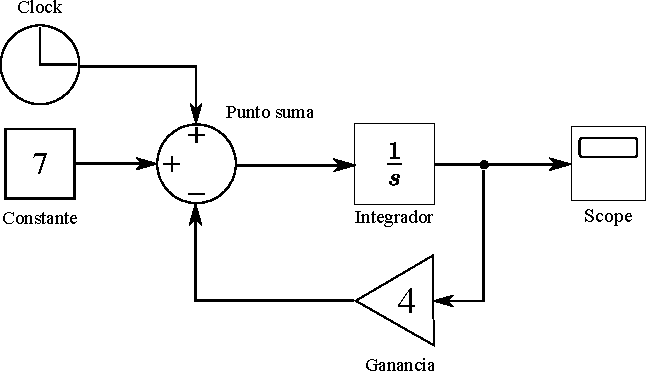
\includegraphics[width = 0.7\textwidth]{imagenes/diagrama_en_bloque2.pdf}
    \caption{Diagrama en bloque de la ecuación diferencial.}
    \label{fig:3}
\end{figure}


Para implementar el sistema 

\begin{equation*}
    \ddot{x}(t) + 2\dot{x}(t) + 3x(t) = \sin t
\end{equation*}

\noindent Despejamos $\ddot{x}$ de la ecuación. Por lo tanto

\begin{equation*}
    \ddot{x}(t)  = \sin t - 2\dot{x}(t) - 3x(t)
\end{equation*}

\noindent donde $\sin t = u(t)$ es la entrada al sistema. En la figura \ref{fig:4} se muestra el diagrama en bloque de dicho sistema.


\begin{figure}[ht!]
    \centering
    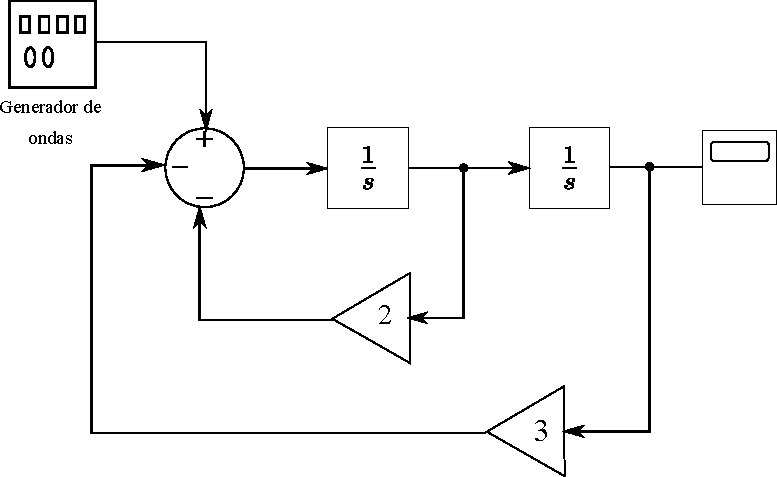
\includegraphics[width = 0.7\textwidth]{imagenes/diagrama_en_bloque3.pdf}
    \caption{Diagrama en bloque de la ecuación diferencial de segundo orden con entrada sinusoidal.}
    \label{fig:4}
\end{figure}



Dado el sistema:

\begin{equation*}
    \ddot{x}(t) + 11\dot{x}(t) + 13x(t) = \dot{r}(t) + 2r(t)
\end{equation*}

\noindent Tomando la transformada de Laplace a ambos miembros:

\begin{equation*}
    \mathcal{L}\{\ddot{x}(t) + 11\dot{x}(t) + 13x(t) = \dot{r}(t) + 2r(t)\}
\end{equation*}

\noindent Se sabe que $\mathcal{L}\{\ddot{x}\} = s^2X(s) - sx(0) - \dot{x}(0)$. Si las condiciones iniciales del sistema son nulas, se obtiene:

\begin{align*}
    &s^2 X(s) + 11 s X(s) + 13 X(s) = sR(s) + 2R(s)\\
    &X(s)(s^2 + 11s + 13) = R(s)(s + 2)
\end{align*}


\noindent Por lo tanto la función de transferencia es:

\begin{equation*}
    \frac{X(s)}{R(s)} = \frac{s + 2}{s^2 + 11s + 13}
\end{equation*}


\noindent La estabilidad del sistema se evalúa mediante el criterio de Routh. Sea el polinomio $s^2 + 11s + 13$, entonces

\begin{align*}
    &s^2 \quad 1 \quad 13 \\
    &s^1 \quad 11 \quad 0 \\
    &s^0  \frac{11\cdot 13 - 1\cdot 0}{11} = 13 > 0
\end{align*}


\noindent Como no hay un cambio de signo, entonces el sistema es estable ante cualquier entrada. La siguiente figura muestra el diagrama en bloques del sistema


\begin{figure}[ht!]
    \centering
    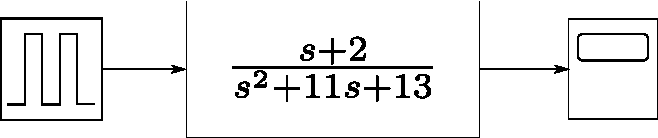
\includegraphics[width = 0.7\textwidth]{imagenes/diagrama_en_bloque4_FT.pdf}
    \caption{Diagrama en bloque para la función de transferecia con entrada pulso.}
    \label{fig:5}
\end{figure}



Sea la ecuación diferencial:

\begin{equation*}
    \ddot{x}(t) + 5x(t) = r(t)
\end{equation*}


\noindent La función transferencia es:


\begin{equation*}
    \frac{X(s)}{R(s)} = \frac{1}{s^2 + 5}
\end{equation*}


\noindent Dado que el polinomio $s^2 + 5$ tiene dos polos conjugados con parte real nula, el sistema es oscilatorio. La respuesta está acotada pero se consideraría inestable para una entrada escalón. La siguiente figura muestra el diagrama en bloque del sistema en \textit{Simulink}\textregistered\ y su salida en conjunto con la entrada.

\begin{figure}[ht!]
    \centering
    \begin{subfigure}{0.48\textwidth}
        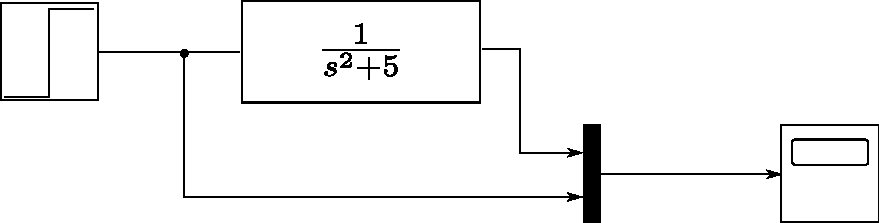
\includegraphics[width = \textwidth]{imagenes/diagrama_en_bloque5.pdf}
        \label{fig:5.1}
        \caption{Diagrama en bloque.}
    \end{subfigure}
    \begin{subfigure}{0.48\textwidth}
        \label{fig:5.2}
        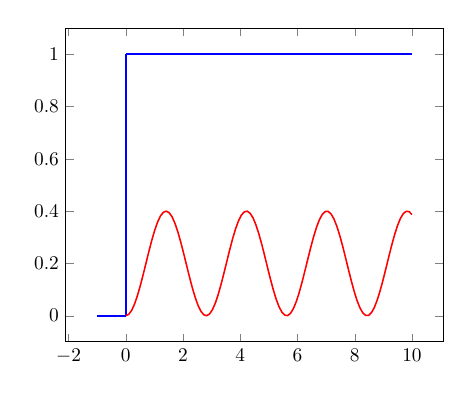
\begin{tikzpicture}[scale = 0.7]
            \begin{axis}[trig format = rad]
                \addplot[domain = -1:0, blue, thick]{0};
                \addplot[domain = 0:10, blue, thick]{1};
                \draw[blue, thick] (axis cs: 0, 0) -- (axis cs: 0, 1);
                \addplot[red, domain = 0:10, samples = 100, thick]{1/5 * (1 - cos(sqrt(5)*x))};
            \end{axis}
        \end{tikzpicture}
        \caption{Salida del sistema.}
    \end{subfigure}
    \caption{Diagrama en bloque (en negro el bloque \textit{Mux}) y respuesta del sistema. En azul la entrada y en rojo la respuesta ante la entrada escalón.}
\end{figure}



Por último, comparemos las siguientes ecuaciones diferenciales:

\begin{center}
    \begin{cases}
        3\ddot{x}(t) + 10\dot{x}(t) + 5x(t) = 5r(t)\\
        \ddot{y}(t) + \dot{y}(t) + y(t) = r(t)
    \end{cases}
\end{center}


\noindent Las funciones transferencias de las siguientes ecuaciones son:

\begin{equation*}
    \frac{X(s)}{R(s)} = \frac{5}{3s^2 + 10s + 5} \qquad \frac{Y(s)}{R(s)} = \frac{1}{s^2 + s + 1}
\end{equation*}

\newpage

\noindent Si $R(s) = 1/s$ (entrada escalón), sus respuestas son:

\begin{figure}[ht!]
    \centering
    \begin{tikzpicture}
        \begin{axis}[xlabel = {$t[s]$},
            ylabel = {$x(t), \ y(t)$},
            grid,
            legend entries = {$x(t)$, $y(t)$, Escalón},
            legend pos = south east]
            \addplot[each nth point=4, thick, red] table[x = t, y = y1]{archivostxt/respuestas.txt};
            \addplot[each nth point=4, thick, cyan] table[x = t, y = y2]{archivostxt/respuestas.txt};
            \addplot[black, thick, domain = 0:20]{1};
            \draw[thick, black] (axis cs: 0, 0) -- (axis cs: 0, 1);
        \end{axis}
    \end{tikzpicture}
    \caption{Salidas de los sistemas por una respuesta escalón}
    \label{fig:7}
\end{figure}



Se observa a simple vista que las respuestas de $x(t)$ y de $y(t)$ tiene un tiempo de asentamiento iguales, con la diferencia que $y(t)$ tiene una sobreenlongación, es decir se trata de un sistema subamortiguado. El sistema $x(t)$ llega al valor final tiempo después que el otro sistema pero sin oscilación. Por lo tanto, si se desea un sistema que no oscile el sistema $x(t)$ es el mejor. 



\newpage

\section{Guía 02}

La siguiente figura representa el modelo del sistema de la guía 02.

\begin{figure}[ht!]
    \centering
    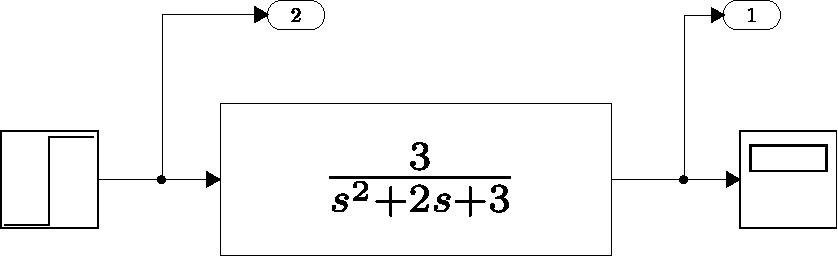
\includegraphics[width = 0.7\textwidth]{imagenes/diagrama_en_bloques_guia02.pdf}
    \caption{Diagrama en bloques del modelo}
    \label{fig:8}    
\end{figure}



Al correr el sistema en Simulink, en el \textit{Workspace} aparece la variable \textit{out}. Para graficar dicho sistema con su entrada se accede a los elementos de la variable out mediante el acceso por punto. El siguiente código de Matlab ejecuta el ploteo de la entrada y salida del sistema.




\begin{figure}[ht!]
\begin{lstlisting}[caption={Extracción de datos y graficado en MATLAB}, label={lst:matlab_plot}]
% Extracción de datos del Timetable
Tabla_1 = out.yout.extractTimetable;
t1 = Tabla_1.Time;
y1 = Tabla_1.Data;
y2 = Tabla_1.Data_1;

% Graficado de resultados
figure;
plot(t1, y1) % Respuesta
hold on; 
plot(t1, y2) % Entrada
\end{lstlisting}
\end{figure}



La ventaja con la que corre el comando \textit{plot} al scope es que es totalmente personalizable pasando únicamente los argumentos necesarios, representando los resultados de una forma más prolija. La desvantaja es que a medida que queremos evaluar distintas entradas al sistema, necesitamos declarar variables el cual puede resultar engorroso. Sin embargo, con el bloque scope se puede lograr una visualización más rápida y menos tediosa. 



\newpage

\section{Lecciones aprendidas y conclusión}
En el siguiente informe se ha desarrollado y aprendido sobre cómo manejar la herramienta Simulink para modelar modelos simples mediante ecuaciones diferenciales (integradores) y funciones de transferencias para distintos tipos de entradas. Se concluye que la herramienta de Simulink es una excelente interfaz entre el usuario y el programa para poder simular y modelar distintos sistemas.



\end{document}